
%runtimes: median - mean - response
In this section we will study the query runtime distributions of different approaches for dealing with Linked Data at scale. In the figures both the \emph{median} and \emph{mean query runtimes} are reported. As the runtime distributions can be skewed, performance differences between systems are most often reported using the median runtime. 

If we consider an ETL~\cite{ETL} process, or equivalently a batch of queries, the mean runtime is more meaningful, as it directly translates to the total batch runtime. In the following box plots we chose to report both.

%response times
Some of the stores provide query results in a streaming fashion. Response times are not captured in the current query event format but are captured in the SPARQL benchmarker summary CSV-files. For GraphDB and Blazegraph the response times are respectively 27\% and 21\% lower than the mean runtimes on WatDiv1000M. For the other engines the difference was close to zero.
%N1_64_Opt WatDiv 1000M: 
%Store 			Avg Mix Response 	Avg Mix Runtime
%Blazegraph: 	7436.614781577 		9361.074445217   	=> 1925 sneller = 21% lager
%Es 			45543.319632289	    45548.207560219  	=> coincide
%GraphDB   		6095.473343756 		8377.37145798 		=> 2282 sneller = 27% lager
%Virtuoso       1984.603994124	    2021.146539186		=> coincide
% LdF1 en LDF3 											=> coincide

%errors excluded
A major concern when comparing query runtime between different engines is \emph{query completeness}. The current query event format, shown in Table~\ref{table:queryevents}, explicitly reports whether a query was solved correctly, meaning it has retrieved the complete set of results. Query completeness is the topic of section~\ref{subsec:completeness}. To interpret the results in this section correctly, it is important to understand that queries, which have incomplete results for at least one benchmark, are completely discarded in the runtime comparisons.

\begin{table}[ht!]
	\centering
	\caption{Conventions for describing benchmark setups.}
	\label{table:namingconv}
	\scalebox{0.9}{
		\begin{tabular}{l|l}
			\hline
			\textbf{Shorthand} & \textbf{Full Description} \\
			\textbf{Notation}	& \; \\
			\hline
			\textbf{Vir1\_32\_Def}                  & Virtuoso - single node - 32GB RAM - \\
			& Default Configuration\\
			\textbf{TPF3\_64\_Def}                  & Triple Pattern Fragments - 3 slave nodes - 64GB RAM - \\
			& Default Configuration\\
			\textbf{Gra1\_64\_Opt}                  & GraphDB - single node - 64GB RAM - \\
			& Optimized (RFI) Configuration\\
			\hline
		\end{tabular}
	}
	 \caption*{A description consists of a 3-character prefix describing the RDF storage solution, the number of nodes, the amount of memory and the configuration.}
\end{table}

%Benchmark Survival
Finally, a subtle error can be made in query runtime comparison for benchmarks which involve a query engine that becomes unresponsive (engine failure). In the runtime comparisons we only consider the range between the first query and the last successful query. We coin this the \emph{benchmark survival interval}.

In Table~\ref{table:namingconv} we introduce a naming convention to describe the different benchmark setups. 

\subsection{Increasingly Large Datasets}
\label{subsec:bigdata}
%
%RESULTS Rev1: Notebook Rev1_13 - A Median & Average Runtime
%RESULTS Rev1: Notebook Rev1_13 - B Errors & Timeout percentage
%
The previous benchmark results~\cite{de2016big} stem from the \emph{None} configuration. In this section however, we use the \emph{Default} configuration of the \emph{Vendor} systems.
In Figure~\ref{fig:Fig01_WatdivNoSQLDataScaling} query runtime distributions are shown for the 4 \emph{Vendor} systems for three different dataset sizes of the WatDiv benchmark: 10M, 100M, and 1000M (million) triples. Note that for these benchmark runs we used a setup with 32 GB memory.
%
%median/mean
%Bla_N1_32_W10_Def    0.033637		0.058546
%Gra_N1_32_W10_Def    0.007062		0.036882
%Es_N1_32_W10_Def     0.163703		0.290875
%Vir_N1_32_W10_Def    0.007511		0.018063
%
%Bla_N1_32_W100_Def   0.191359		0.461707
%Gra_N1_32_W100_Def   0.047812		0.417214
%Es_N1_32_W100_Def    48.305706		72.994550
%Vir_N1_32_W100_Def   0.046707		0.301350
%  
%Bla_N1_32_W1000_Def  8.858862 		56.437824
%Gra_N1_32_W1000_Def  47.932701 	74.927924
%Es_N1_32_W1000_Def   64.217677 	121.887237
%Vir_N1_32_W1000_Def  0.258209  	5.622635
%speedups
%Bla		7.8862262153 		122.2373150071
%Gra		11.3121305786 		179.5911067222
%Es			250.9481736141 		1.6698128422
%Vir		16.6832752035 		18.6581549693

\begin{itemize}
	\item \textbf{Runtime vs Dataset Size:} Although only 3 data points are available for 10, 100 and, 1000M triples, it is interesting to investigate how the runtime scales when the dataset grows by a factor 10. If we focus on the average query runtimes (dots) two trends can be observed: \textbf{Vir1\_32} has a nearly constant multiplication factor (mf) while for the other stores this is not the case. Going from 10M to 100M the mfs are 8, 11, and 17 for \textbf{Bla1\_32}, \textbf{Gra1\_32}, and \textbf{Vir1\_32} respectively. Going from 100M the mf for \textbf{Vir1\_32} is 19, but for the other systems mf $> 120$! A possible explanation for this trend break is that memory swapping occurs. This observation motivates the choice for 64GB memory instances as the central reference setup from which to explore the benchmark space.
%errors and timeouts
%Bla_N1_32_W1000_Def:	Success: 88.3	Error: 0.0	Timeout: 11.6
%Gra_N1_32_W1000_Def:	Success: 100.	Error: 0.0	Timeout: 0.0
%Es_N1_32_W1000_Def:	Success: 67.2	Error: 0.0	Timeout: 32.7
%Vir_N1_32_W1000_Def:	Success: 99.9	Error: 0.04	Timeout: 0.0
\item \textbf{Timeouts \& Errors:} Most of the queries are executed successfully by all \emph{Vendor} systems. For WatDiv1000M \textbf{Bla1\_32} already has a timeout percentage of 11.6\% and for \textbf{ES1\_32} this is even 32.7\%. Note however that these results do not affect the plots as we only use query events from the \emph{benchmark survival interval}. 
\item \textbf{GraphDB vs Virtuoso:} In terms of median runtime both \textbf{Gra1\_32} and \textbf{Vir1\_32} are tied at 0.01s and 0.05s in the two leftmost panels of Fig.~\ref{fig:Fig01_WatdivNoSQLDataScaling}. With sufficient memory these engines can remain competitive. However, for 1000M dataset only \textbf{Vir1\_32} is performing well, with an increase in median runtime with a factor of 18.6 compared to 100M run while the median runtimes of the other stores increase with a factor of 100 or more. 
\textbf{Gra\_32}, more than the other stores, suffers from a long tail which has a major effect on the average runtimes for WatDiv10M and 100M. If we compare these runtimes, Virtuoso is 1.5-2 times faster.

\item \textbf{Blazegraph vs. GraphDB:} \textbf{Bla1\_32} competes with \textbf{Gra1\_32} in terms of average runtimes but not in terms of median runtimes.

\item \textbf{ES consistently last:} \textbf{ES\_32}, even on WatDiv10M, lags by a factor of at least 5 to the other systems. For WatDiv100M already the nonlinear scaling behavior sets in, making it the only engine to experience problems with the 100M dataset. 
\end{itemize}
%


\subsection{Vertical Scaling}
\label{subsec:vscaling}
%
%RESULTS Rev1: Notebook Rev1_13 - A Median & Average Runtime

%
%RESULTS Rev1: Notebook Rev1_13 - B Errors & Timeout percentage
%
In the previous section we observed that the amount of memory is a critical parameter for benchmark performance. 
In this section we study the effect on query runtimes by increasing memory to 64GB.
The two leftmost panels of Fig.~\ref{fig:Fig02_WatdivVerticalScaling} study the effect of vertical scaling. 
%median / mean
%Bla_N1_32_W1000_Def     8.858862	56.437824
%Gra_N1_32_W1000_Def    47.932701	74.927924
%Es_N1_32_W1000_Def     64.217677	121.887237
%Vir_N1_32_W1000_Def     0.258209	5.622635
%
%Bla_N1_64_W1000_Def     2.825023	6.741764
%Gra_N1_64_W1000_Def    40.375218	59.564284
%Es_N1_64_W1000_Def     35.178332	103.637674
%Vir_N1_64_W1000_Def     0.175917	3.667321
%speedups
%Bla_N1_64_W1000_Def     3	10
%Gra_N1_64_W1000_Def     1  1 
%Es_N1_64_W1000_Def      2  
%Vir_N1_64_W1000_Def     1

\begin{itemize}
	\item \textbf{Memory is no magic solution:} Especially for \textbf{Gra1\_64\_Def} and \textbf{Vir1\_64\_Def} hardly any improvement can be observed. Blazegraph takes full advantage of the additional memory, with a large shift in both median and mean runtimes. %The strong hardware dependence of Blazegraph could be a motivation to also study the performance in a GPU setting~\cite{blazegraphgpu}, which is outside the scope of this work.
	\item \textbf{Speedups:} \textbf{Bla1\_64\_Def} has a speedup of 8.4 for its average runtime and 3.1 for its median runtime. For the other stores only \textbf{ES1\_64\_Def} benefits with a speedup of 1.8 for its average runtime.
	%\item \textbf{Benefits for fast queries:} The most outspoken positive effect is the lowering of the lower boundary of the box plots.  
\end{itemize}

%FIGURES ORIGAL PAPER
%FIG_BenchmarkSurvival
%\begin{figure}[ht!]
%	\centering
%	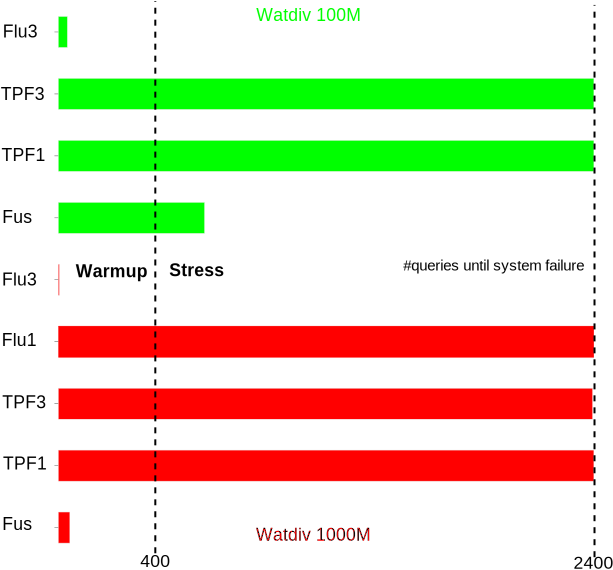
\includegraphics[width=0.99\linewidth]{imgs/F2_BenchmarkSurvival_Other_Reworked}
%	\caption{Benchmark survival for other systems. \textbf{TPF} stays operational for both WatDiv1000M and WatDiv100M. Both as an approach to handle compressed data (\textbf{TPF1})
%		as an approach to support query federation (\textbf{TPF3}) it fulfills its promise of high availability. As of the other approaches only \textbf{Fus} gets passed the warmup phase for WatDiv100M.}
%	\label{fig:F2_BenchmarkSurvival_Other_Reworked}
%\end{figure}
%FIG_ScalingNoSQL
%\begin{figure*}[!ht]
%	\centering
%	\includegraphics[width=0.99\linewidth]{imgs/F6_Scaling_NoSQL_WatDiv1000M_Reworked.eps}
%	\caption{Four panels showing the effect of adding more RAM and \emph{optimized} configurations on the query runtime distribution for WatDiv1000M. In the \emph{optimized} setting Blazegraph and GraphDB share second place. Virtuoso outperforms the other stores even in the 32GB, \emph{default} setup. Adding more memory doesn't impact its performance implying that it doesn't require extra resources. For GraphDB the effect of proper configuration is the most extreme, its performance strongly depends on turning on the correct indexes.}
%	\label{fig:F6_Scaling_NoSQL_WatDiv1000M_Reworked}
%	%\rv{Always name the axes also inside of the figure. I know it's in the caption, but \emph{some} reviewer \emph{will} nag about it.}
%\end{figure*}


\subsection{RFI: Optimized Configurations}
\label{subsec:rfi}
%
%RESULTS Rev1
%RUNTIME
%SUCCESS/ERROR

%Convergence of results? Not with memory, with configs though...
After contacting the vendors with our initial results one of the parties suggested to demonstrate the optimal operation of their database. 
This was formalized by sending out a Request-For-Information (RFI), specifying the benchmarks we were planning to run.
3 out of 4 vendors chose to participate in the RFI, which resulted in an \emph{Optimized} configuration. 

In Figure~\ref{fig:Fig02_WatdivVerticalScaling} the rightmost panel corresponds to running the benchmark with the \emph{Optimized} configuration.

%
%median/mean
%Bla_N1_64_W1000_Def     2.825023 	6.741764
%Gra_N1_64_W1000_Def    40.375218 	59.564284
%Vir_N1_64_W1000_Def     0.175917 	3.667321
%
%Bla_N1_64_W1000_Opt    0.739366 	1.945429
%Gra_N1_64_W1000_Opt    0.652474  	6.320693
%Vir_N1_64_W1000_Opt    0.167420 	4.054050
%
\begin{itemize}
	\item \textbf{Sensitivity to configuration:} \textbf{Vir1\_64} got no benefit from the RFI settings file. For 
	\textbf{Bla1\_64} the only improvement was to explicitly configure the timeout parameter on the server side. This avoids unnecessary overhead while the client is already disconnected. It leads to a speedup of approximately 3.5 for both runtime measurements. \textbf{Gra1\_64} has the highest sensitivity to proper configurations. The provided scripts ensure a batch speedup of 9.4 and a median runtime speedup of 62.
	\item \textbf{32\_Def to 64\_Opt:} Moving from the left panel to the right in Figure~\ref{fig:Fig02_WatdivVerticalScaling}, we clearly see results converging. \textbf{Bla1\_64} is the most efficient system for processing batch workloads with an average runtime of 1.95s per query, 4.05s and 6.32s for \textbf{Vir1\_64} and \textbf{Gra1\_64} respectively. In the query performance \textbf{Vir1\_64} has a median runtime of 0.17s where \textbf{Gra1\_64} and \textbf{Bla1\_64} have runtimes of 0.65s and 0.74s respectively.
%Bla_N1_32_W100_Def   0.191359		0.461707	=> x5
%Gra_N1_32_W100_Def   0.047812		0.417214 	=> x15
%Vir_N1_32_W100_Def   0.046707		0.301350	=> x15
	\item \textbf{Runtime vs Dataset Size:} Returning to section~\ref{subsec:bigdata} we can verify that the linear scaling behavior is largely restored, confirming our earlier hypothesis. Multiplication factors drop to 4.2 for Blazegraph, for Virtuoso and GraphDB mf $ \approx 15$.
\item \textbf{Timeouts \& Errors:} Apart from 5\% timeouts for \textbf{Gra1\_64\_Opt}, no query errors are observed with the \emph{Optimized} configurations.
\end{itemize}
%Bla_N1_64_W1000_Opt:	Success: 100.	Error: 0.0	Timeout: 0.0
%Gra_N1_64_W1000_Opt:	Success: 95.0	Error: 0.0	Timeout: 5.0
%Vir_N1_64_W1000_Opt:	Success: 100.	Error: 0.0	Timeout: 0.0



\subsection{Semantic Web Solutions}
\label{subsec:semweb}
%
%RESULTS Rev1: Notebook Rev1_13 - A Median & Average Runtime
%median/mean
%LdF_N1_64_W100_Def     19.949113	64.842078
%LdF_N3_64_W100_Def     58.365978 	122.960265
%LdF_N1_64_W1000_Def    300.0		219.935204
%LdF_N3_64_W1000_Def    300.0		216.525390
%
%RESULTS Rev1: Notebook Rev1_13 - B Errors & Timeout percentage
%Fus_N1_64_W100_Def:	Success: 65.0	Error: 0.0	Timeout: 34.9
%FedX_N3_64_W100_Def:	Success: 0.0	Error: 0.0	Timeout: 0.0
%LdF_N1_64_W100_Def:	Success: 89.0	Error: 0.0	Timeout: 10.9
%LdF_N3_64_W100_Def:	Success: 75.2	Error: 0.0	Timeout: 24.7
%
%Fus_N1_64_W1000_Def:	Success: 0.0	Error: 0.0	Timeout: 0.0
%FedX_N1_64_W1000_Def:	Success: 95.0	Error: 0.0	Timeout: 5.0
%FedX_N3_64_W1000_Def:	Success: 0.0	Error: 0.0	Timeout: 0.0
%LdF_N1_64_W1000_Def:	Success: 28.8	Error: 0.0	Timeout: 71.1
%LdF_N3_64_W1000_Def:	Success: 29.3	Error: 0.0	Timeout: 70.6
%

%As the initial goal of the research collaboration with Ontoforce was to find a solution to work with federated querying on top of live data sources on the Semantic Web, 
In this section we discuss the results of \textbf{Fus1\_64}, \textbf{FedX3\_64}, \textbf{TPF1\_64} and \textbf{TPF3\_64}. 
For these 3 systems engine failure and query errors are very common with only the \textbf{TPF*\_64} systems surviving the entire benchmark.
Fig.~\ref{fig:Fig03_BenchmarkSurvival_Other_Watdiv_Default} shows the \emph{Benchmark Survival Interval}, defined as the range between the first and the last successful query. 
Given the high degree of failures we do not show the query runtime results.
%Note however that these results do not affect the plots as we only use query events from the \emph{benchmark survival interval}. 
%Fig. deliberately has no relation with query runtimes. 

%Benchmark Survival
%Finally, a subtle error can be made in query runtime comparison for benchmarks which involve a query engine that becomes unresponsive (engine failure). In the runtime comparisons we only consider  We name this the \emph{benchmark survival interval}, this is shown in Figure~\ref{fig:Fig03_BenchmarkSurvival_Other_Watdiv_Default}.

\begin{itemize}
	\item \textbf{FedX1\_64:} This single-node setup is tested to verify whether FedX manages to parse the queries. As the queries have the same form for WatDiv100M we only tested this in the 1000M setting.
	\item \textbf{Specific Templates cause crashes:} Where \\ \textbf{TPF*\_64} systems more gracefully timeout on the \textbf{C} templates, \textbf{C2} causes a crash in \textbf{Fus1\_64} and \textbf{C3} in \textbf{FedX3\_64}, upon their first occurrence in warm-up or stress run. \textbf{C3} is a query with very low triple pattern selectivity leading to large in-memory joins.
	\item \textbf{Crash investigation:} For \textbf{FedX3\_64} the benchmark was terminated after running into constant timeouts for 8 hours. Inspection of the slave nodes showed them to be idle, while the federator node had its entire memory pool saturated, with the CPU load close to zero. This might be related to issues with garbage collection.
	For \textbf{Fus1\_64} after a number of queries a continuous timeout sequence sets in. The specific HDT implementation for Fuseki ignores the timeout parameter. This might explain why the server became unresponsive.
	\item \textbf{Staying alive:} \textbf{TPF*\_64} survive both WatDiv benchmarks, nonetheless with up to 71\% of the queries timeouts on WatDiv1000M. On WatDiv100M the timeout ratio drops to 25\% for \textbf{TPF3\_64} and to 11\% for \textbf{TPF1\_64}.
%Fus_N1_64_W100_Def:	Success: 65.0	Error: 0.0	Timeout: 34.9
%FedX_N3_64_W100_Def:	Success: 0.0	Error: 0.0	Timeout: 0.0
%LdF_N1_64_W100_Def:	Success: 89.0	Error: 0.0	Timeout: 10.9
%LdF_N3_64_W100_Def:	Success: 75.2	Error: 0.0	Timeout: 24.7
%
%Fus_N1_64_W1000_Def:	Success: 0.0	Error: 0.0	Timeout: 0.0
%FedX_N1_64_W1000_Def:	Success: 95.0	Error: 0.0	Timeout: 5.0
%FedX_N3_64_W1000_Def:	Success: 0.0	Error: 0.0	Timeout: 0.0
%LdF_N1_64_W1000_Def:	Success: 28.8	Error: 0.0	Timeout: 71.1
%LdF_N3_64_W1000_Def:	Success: 29.3	Error: 0.0	Timeout: 70.6
	\item \textbf{Runtime Comparison: } Only for WatDiv100M comparing the runtimes of \textbf{TPF*\_64} to the \emph{Vendor} systems is meaningful due to the higher query success rates. Compared to \textbf{ES1\_32}, the \textbf{TPF1\_64} is 2.4 times faster in terms of median runtime and 12\% in terms of average runtime. For \textbf{TPF3\_64} the results are worse than \textbf{ES1\_32}: 25\% slower in median runtime, 40\% slower for average runtime.
\end{itemize}
%Bla_N1_32_W100_Def   0.191359		0.461707
%Gra_N1_32_W100_Def   0.047812		0.417214
%Es_N1_32_W100_Def    48.305706		72.994550
%Vir_N1_32_W100_Def   0.046707		0.301350
%LdF_N1_64_W100_Def     19.949113	64.842078
%LdF_N3_64_W100_Def     58.365978 	122.960265











\subsection{Horizontal scaling}
\label{subsec:hscaling}
%
%RESULTS Rev1: Notebook Rev1_13 - A Median & Average Runtime
%
%median/mean
%Vir_N1_32_W1000_Def    0.295139	4.431931
%Vir_N3_32_W1000_Def    1.040609	8.545433
%
%Es_N1_32_W1000_Def     74.091186 	132.011802
%Es_N3_32_W1000_Def    300.000000 	191.478380
%   
%LdF_N1_64_W1000_Def    300.0 		219.935204
%LdF_N3_64_W1000_Def    300.0		216.525390
%
%RESULTS Rev1: Notebook Rev1_13 - B Errors & Timeout percentage
%Bla_N1_32_W10_Def:	Success: 100.	Error: 0.0	Timeout: 0.0
%Gra_N1_32_W10_Def:	Success: 100.	Error: 0.0	Timeout: 0.0
%Es_N1_32_W10_Def:	Success: 100.	Error: 0.0	Timeout: 0.0
%Vir_N1_32_W10_Def:	Success: 100.	Error: 0.0	Timeout: 0.0
%
%Bla_N1_32_W100_Def:	Success: 100.	Error: 0.0	Timeout: 0.0
%Gra_N1_32_W100_Def:	Success: 100.	Error: 0.0	Timeout: 0.0
%Es_N1_32_W100_Def:	Success: 100.	Error: 0.0	Timeout: 0.0
%Vir_N1_32_W100_Def:	Success: 100.	Error: 0.0	Timeout: 0.0
%
%Bla_N1_32_W1000_Def:	Success: 88.3	Error: 0.0	Timeout: 11.6
%Gra_N1_32_W1000_Def:	Success: 100.	Error: 0.0	Timeout: 0.0
%Es_N1_32_W1000_Def:	Success: 67.2	Error: 0.0	Timeout: 32.7
%Vir_N1_32_W1000_Def:	Success: 99.9	Error: 0.04	Timeout: 0.0
%
%Bla_N1_64_W1000_Def:	Success: 95.0	Error: 0.0	Timeout: 5.0
%Gra_N1_64_W1000_Def:	Success: 79.6	Error: 0.0	Timeout: 20.4
%EsS_N1_64_W1000_Def:	Success: 72.5	Error: 0.0	Timeout: 27.4
%Vir_N1_64_W1000_Def:	Success: 100.	Error: 0.0	Timeout: 0.0
%
%Bla_N1_64_W1000_Opt:	Success: 100.	Error: 0.0	Timeout: 0.0
%Gra_N1_64_W1000_Opt:	Success: 95.0	Error: 0.0	Timeout: 5.0
%Vir_N1_64_W1000_Opt:	Success: 100.	Error: 0.0	Timeout: 0.0
%
%Es_N3_32_W1000_Def:	Success: 34.8	Error: 65.1	Timeout: 0.0
%Vir_N3_32_W1000_Def:	Success: 100.	Error: 0.0	Timeout: 0.0
%
%Fus_N1_64_W100_Def:	Success: 65.0	Error: 0.0	Timeout: 34.9
%Flu_N3_64_W100_Def:	Success: 0.0	Error: 0.0	Timeout: 0.0
%LdF_N1_64_W100_Def:	Success: 89.0	Error: 0.0	Timeout: 10.9
%LdF_N3_64_W100_Def:	Success: 75.2	Error: 0.0	Timeout: 24.7
%
%Fus_N1_64_W1000_Def:	Success: 0.0	Error: 0.0	Timeout: 0.0
%Flu_N1_64_W1000_Def:	Success: 95.0	Error: 0.0	Timeout: 5.0
%Flu_N3_64_W1000_Def:	Success: 0.0	Error: 0.0	Timeout: 0.0
%LdF_N1_64_W1000_Def:	Success: 28.8	Error: 0.0	Timeout: 71.1
%LdF_N3_64_W1000_Def:	Success: 29.3	Error: 0.0	Timeout: 70.6
%
%Bla_N1_64_Ont_Opt:	Success: 0.0	Error: 0.0	Timeout: 0.0
%Es_N1_64_Ont_Def:	Success: 57.6	Error: 22.2	Timeout: 20.0
%Gra_N1_64_Ont_Opt:	Success: 45.0	Error: 0.0	Timeout: 54.9
%Vir_N1_64_Ont_Opt:	Success: 98.7	Error: 0.67	Timeout: 0.58
%Vir_N1_32_Ont_Opt_VWall:	Success: 98.8	Error: 0.67	Timeout: 0.50
%Vir_N3_64_Ont_Opt_0:	Success: 95.8	Error: 3.71	Timeout: 0.45
%Vir_N3_64_Ont_Opt_2:	Success: 86.0	Error: 13.9	Timeout: 0.0
%
%


An alternative to increasing the memory in a single-node server is to increase the overall resources by 
adding more nodes, thus creating a distributed system. 

All 4 commercial RDF solutions support multi-node setups. GraphDB however, works only as a HA-solution (High-Availability): we did not evaluate this approach since 
it requires all data to be replicated on every node and does not support data partitioning, which is required to scale beyond the single-node resource limits.
The performance can however be estimated since it is equivalent to a setup with N identical databases with a load balancer equally distributing the queries between
the database replicas. The effect is a linear speedup in terms of completing a full query-mix. 
Virtuoso also supports a similar setup.
The effect on the individual query runtimes should be limited, but not completely absent since the database load on the individual nodes will be smaller. The effect of database load on the query runtimes will be studied in the next section.


For Blazegraph, support was required for setting up the multi-node system. This support was requested via the RFI but not fulfilled, which limited our comparison to \textbf{Vir3\_32\_Def}, \textbf{ES3\_32\_Def}, and \textbf{TPF3\_64\_Def}.

Fig.~\ref{fig:Fig04_WatdivHorizontalScaling} shows pairwise comparisons of the three setups for which we have both a single and a 3-node benchmark. 

\begin{itemize}
	\item \textbf{Benchmark survival interval:} %[('ES_N3_32_W1000_Def', 8684), ('Vir_N3_32_W1000_Def', 12000)]
	\textbf{Vir3\_32\_Def} and \textbf{TPF3\_64\_Def} managed to stay online during the entire Watdiv1000M benchmark, whereas \textbf{ES3\_32\_Def} stopped responding after having completed 67\% of the multi-threaded run. 
	%Es_N3_32_W1000_Def:	Success: 34.8	Error: 65.1	Timeout: 0.0
	%Vir_N3_32_W1000_Def:	Success: 100.	Error: 0.0	Timeout: 0.0
	\item \textbf{Errors \& Timeouts:} 65\% of the queries of \textbf{ES3\_32\_Def} resulted in an HTTP 504 error, mentioning \textit{Gateway Timeout}. Further study revealed that this timeout was due to an internal configuration parameter in the ES distributed setup, unfortunately we did not receive any feedback on this issue. \textbf{Vir3\_32} successfully completed all queries. 70.6\% of the queries result in a timeout for \textbf{TPF3\_64\_Def}.
	\item \textbf{Multi-node overhead:} For all setups additional nodes lead to overhead instead of speedup. Runtime MFs are 1.9 and 1.5 for \textbf{Vir} and \textbf{ES}. \textbf{TPF} has a negligible overhead but is already very close to the query timeout.
\end{itemize}
%query_events_correct => double check on crash!
%Es: (Virtuoso 12k = all, TPF_64 also all)
% T1 warmup survival: 	2000
% T stress: 1343 - 1331 - 1348 - 1320 - 1348
%median/mean
%Vir_N1_32_W1000_Def    0.295139	4.431931
%Vir_N3_32_W1000_Def    1.040609	8.545433
%
%Es_N1_32_W1000_Def     74.091186 	132.011802
%Es_N3_32_W1000_Def    300.000000 	191.478380
%   
%LdF_N1_64_W1000_Def    300.0 		219.935204
%LdF_N3_64_W1000_Def    300.0		216.525390

In a discussion with OpenLink it was clarified that Virtuoso Cluster acts as a \emph{distributed memory solution}. This implies that adding nodes does not lead to a speedup in the query runtimes, but the total of memory pool in the system increases, allowing it to handle larger datasets. Since the single node benchmark did not exhaust the memory, there is no advantage to be expected from a multi-node setup. As an indication, according to support a 32GB machine should be able to manage up to 3 billion triples (10GB per 1B triples). 
This observation, together with the lack of feedback on the issues with \textbf{ES3\_32\_Def} and the high timeout percentage for \textbf{TPF3\_64\_Def} motivated our decision to not run any further multi-node benchmarks..

Systems translating SPARQL queries to distributed platforms such as Hadoop~\cite{cure2015evaluation, graux2016multi} are an alternative approach we did not test. Although these approaches are usually not recommended in a context with low-latency requirements, they are specifically designed to operate in an ETL-setting. 
Results for S2RDF~\cite{Schatzle:2016:SRQ:2977797.2977806}, which uses Apache Spark on Watdiv1000M indicate that a 10-node setup can be close to 10 times faster than a single-node Virtuoso server. Since these SPARQL-on-Hadoop solutions are not sufficiently mature and for example cannot be tested using a SPARQL endpoint, definite conclusions currently can not be drawn. 
%One observation to motivate this caution is the fact that Virtuoso is hardly affected when running multiple benchmark clients at once, as will be shown in section~\ref{subsec:load}. The operational cost for these Hadoop setups can also not immediately be deduced.















